\batchmode
\documentclass[a4paper]{book}
\usepackage{makeidx}
\usepackage{natbib}
\usepackage{graphicx}
\usepackage{multicol}
\usepackage{float}
\usepackage{listings}
\usepackage{color}
\usepackage{ifthen}
\usepackage[table]{xcolor}
\usepackage{textcomp}
\usepackage{alltt}
\usepackage[utf8]{inputenc}
\usepackage{mathptmx}
\usepackage[scaled=.90]{helvet}
\usepackage{courier}
\usepackage{sectsty}
\usepackage[titles]{tocloft}
\usepackage{doxygen}
\lstset{language=C++,inputencoding=utf8,basicstyle=\footnotesize,breaklines=true,breakatwhitespace=true,tabsize=8,numbers=left }
\makeindex
\setcounter{tocdepth}{3}
\renewcommand{\footrulewidth}{0.4pt}
\renewcommand{\familydefault}{\sfdefault}
\hfuzz=15pt
\setlength{\emergencystretch}{15pt}
\hbadness=750
\tolerance=750
\begin{document}
\begin{titlepage}
\vspace*{7cm}
\begin{center}
{\Large wifi\-\_\-scan }\\
\vspace*{1cm}
{\large \-Generated by Doxygen 1.7.6.1}\\
\vspace*{0.5cm}
{\small Thu Apr 18 2013 09:29:03}\\
\end{center}
\end{titlepage}
\clearemptydoublepage
\pagenumbering{roman}
\tableofcontents
\clearemptydoublepage
\pagenumbering{arabic}
\chapter{\-Main \-Page}
\label{index}

{\bfseries wifi\-\_\-scan} is a wireless \-Ethernet scanning driver. \-Currently, only the ability to report the received signal strength indication (\-R\-S\-S\-I) of visible access points (\-A\-Ps) is implemented.\section{\-Code A\-P\-I}\label{index_codeapi}
\-The wifi\-\_\-scan code \-A\-P\-I is built so that there are no \-R\-O\-S debug messages being cast internally. \-All exceptions will be thrown, usually as an integer. \-For possible exceptions, see the method documentation.

\-The \-A\-P\-I consists for now out of the \doxyref{\-Wifi\-Scan}{p.}{classWifiScan} class. \-It implements following methods\-:
\begin{DoxyItemize}
\item \doxyref{\-Wifi\-Scan\-::create\-Fingerprint(ros\-::\-Publisher $\ast$pub)}{p.}{classWifiScan_a4232f9f50651eb7fbbb53eebdee48021}
\end{DoxyItemize}\section{\-R\-O\-S A\-P\-I}\label{index_rosapi}
\-List of nodes\-:
\begin{DoxyItemize}
\item {\bfseries fingerprint} 
\end{DoxyItemize}



\subsection{fingerprint}\label{index_fingerprint}
fingerprint publishes a \-R\-S\-S\-I message to the /wifi\-\_\-fp topic.\subsubsection{}\label{_}
\-Since the \-Ethernet interfaces are root restricted, root privileges are necessary to perform valid scans. \-To allow root privileges, follow these steps\-:

\-After compilation, the executable must have its ownership and group changed to root\-:root. \-It is assumed that compilation is done with `catkin`, from the `catkin` project folder. \-Compiled source is assumed to be in the `devel' directory of the working directory. \begin{DoxyVerb}
sudo chown root:root devel/lib/wifi_scan/fingerprint
sudo chmod a+s /devel/lib/wifi_scan/fingerprint
\end{DoxyVerb}
\subsubsection{\-Usage}\label{index_Usage}
\begin{DoxyVerb}
$ rosrun wifi_scan fingerprint [standard ROS args]
\end{DoxyVerb}


\begin{DoxyParagraph}{\-Example}

\end{DoxyParagraph}
\begin{DoxyVerb}
$ rosrun wifi_scan fingerprint wifi_fp:=my_topic
\end{DoxyVerb}
\subsubsection{\-R\-O\-S topics}\label{index_topics}
\-Publishes to\-:
\begin{DoxyItemize}
\item {\bfseries \char`\"{}wifi\-\_\-fp\char`\"{}}\-: [\-Fingerprint] \-List of unique [\-Address\-R\-S\-S\-I] messages. \-This is a pair of device address as string and \-R\-S\-S\-I as float64.
\end{DoxyItemize}\subsubsection{\-R\-O\-S parameters}\label{index_parameters}
\-Reads the following parameters from the command line


\begin{DoxyItemize}
\item {\bfseries \char`\"{}$\sim$topic\char`\"{}} \-: {\bfseries }[string] \-Set the topic to a different value. \-Equal to default \-R\-O\-S renaming capabilities, but less ambiguous. \-Defaults to \char`\"{}wifi\-\_\-fp\char`\"{}.
\item {\bfseries \char`\"{}$\sim$interface\char`\"{}} \-: {\bfseries }[string] \-Set the \-Ethernet interface to scan. \-Defaults to \char`\"{}wlan0\char`\"{}. 
\end{DoxyItemize}
\chapter{\-Class \-Index}
\section{\-Class \-List}
\-Here are the classes, structs, unions and interfaces with brief descriptions\-:\begin{DoxyCompactList}
\item\contentsline{section}{{\bf \-Wifi\-Scan} \\*\-The wifi\-\_\-scan main class }{\pageref{classWifiScan}}{}
\end{DoxyCompactList}

\chapter{\-File \-Index}
\section{\-File \-List}
\-Here is a list of all files with brief descriptions\-:\begin{DoxyCompactList}
\item\contentsline{section}{{\bf fingerprint.\-cpp} }{\pageref{fingerprint_8cpp}}{}
\item\contentsline{section}{{\bf wifiscan.\-cpp} }{\pageref{wifiscan_8cpp}}{}
\item\contentsline{section}{{\bf wifiscan.\-h} }{\pageref{wifiscan_8h}}{}
\end{DoxyCompactList}

\chapter{\-Class \-Documentation}
\section{\-Wifi\-Scan \-Class \-Reference}
\label{classWifiScan}\index{\-Wifi\-Scan@{\-Wifi\-Scan}}


\-The wifi\-\_\-scan main class.  




{\ttfamily \#include $<$wifiscan.\-h$>$}

\subsection*{\-Public \-Member \-Functions}
\begin{Indent}{\bf 01. \-Constructors and destructor}\par
\begin{DoxyCompactItemize}
\item 
{\bf \-Wifi\-Scan} (std\-::string {\bf interface}=\char`\"{}wlan0\char`\"{})
\begin{DoxyCompactList}\small\item\em \-Default constructor. \end{DoxyCompactList}\item 
virtual {\bf $\sim$\-Wifi\-Scan} ()
\begin{DoxyCompactList}\small\item\em \-Destructor. \end{DoxyCompactList}\end{DoxyCompactItemize}
\end{Indent}
\begin{Indent}{\bf 02. \-Configuration}\par
\begin{DoxyCompactItemize}
\item 
std\-::string {\bf interface} () const 
\begin{DoxyCompactList}\small\item\em \-Get the interface on which scans are performed. \end{DoxyCompactList}\item 
void {\bf set\-\_\-interface} (std\-::string {\bf interface})
\begin{DoxyCompactList}\small\item\em \-Set the interface to perform scans on. \end{DoxyCompactList}\end{DoxyCompactItemize}
\end{Indent}
\begin{Indent}{\bf 03. \-R\-O\-S operations}\par
\begin{DoxyCompactItemize}
\item 
void {\bf create\-Fingerprint} (ros\-::\-Publisher $\ast$pub)
\begin{DoxyCompactList}\small\item\em \-Publishes a \-Fingerprint message to the \-Publisher pub. \end{DoxyCompactList}\end{DoxyCompactItemize}
\end{Indent}
\subsection*{\-Private \-Attributes}
\begin{DoxyCompactItemize}
\item 
std\-::string {\bf interface\-\_\-}
\end{DoxyCompactItemize}


\subsection{\-Detailed \-Description}
\-The wifi\-\_\-scan main class. 

\-The \doxyref{\-Wifi\-Scan}{p.}{classWifiScan} class allows for easy operations on the iwlib library, and easy publishing to the defined topics. 

\-Definition at line 44 of file wifiscan.\-h.



\subsection{\-Constructor \& \-Destructor \-Documentation}
\index{\-Wifi\-Scan@{\-Wifi\-Scan}!\-Wifi\-Scan@{\-Wifi\-Scan}}
\index{\-Wifi\-Scan@{\-Wifi\-Scan}!WifiScan@{\-Wifi\-Scan}}
\subsubsection[{\-Wifi\-Scan}]{\setlength{\rightskip}{0pt plus 5cm}{\bf \-Wifi\-Scan\-::\-Wifi\-Scan} (
\begin{DoxyParamCaption}
\item[{std\-::string}]{interface = {\ttfamily \char`\"{}wlan0\char`\"{}}}
\end{DoxyParamCaption}
)}\label{classWifiScan_ae2f428da3fd5a40d584a9b1ddeb7f7a6}


\-Default constructor. 


\begin{DoxyParams}{\-Parameters}
{\em interface} & \-The \-Ethernet interface to scan. \-Defaults to \char`\"{}wlan0\char`\"{}. \\
\hline
\end{DoxyParams}


\-Definition at line 22 of file wifiscan.\-cpp.

\index{\-Wifi\-Scan@{\-Wifi\-Scan}!$\sim$\-Wifi\-Scan@{$\sim$\-Wifi\-Scan}}
\index{$\sim$\-Wifi\-Scan@{$\sim$\-Wifi\-Scan}!WifiScan@{\-Wifi\-Scan}}
\subsubsection[{$\sim$\-Wifi\-Scan}]{\setlength{\rightskip}{0pt plus 5cm}{\bf \-Wifi\-Scan\-::$\sim$\-Wifi\-Scan} (
\begin{DoxyParamCaption}
{}
\end{DoxyParamCaption}
)\hspace{0.3cm}{\ttfamily  [virtual]}}\label{classWifiScan_adb6f0a117e023c829c51088bbb6895c1}


\-Destructor. 



\-Definition at line 27 of file wifiscan.\-cpp.



\subsection{\-Member \-Function \-Documentation}
\index{\-Wifi\-Scan@{\-Wifi\-Scan}!create\-Fingerprint@{create\-Fingerprint}}
\index{create\-Fingerprint@{create\-Fingerprint}!WifiScan@{\-Wifi\-Scan}}
\subsubsection[{create\-Fingerprint}]{\setlength{\rightskip}{0pt plus 5cm}void {\bf \-Wifi\-Scan\-::create\-Fingerprint} (
\begin{DoxyParamCaption}
\item[{ros\-::\-Publisher $\ast$}]{pub}
\end{DoxyParamCaption}
)}\label{classWifiScan_a4232f9f50651eb7fbbb53eebdee48021}


\-Publishes a \-Fingerprint message to the \-Publisher pub. 

\-A fingerprint is a list of all visible \-Wi\-Fi access points' device addresses linked with their corresponding received signal strength indication.


\begin{DoxyParams}{\-Parameters}
{\em pub} & \-A \-R\-O\-S \-Publisher, publishing wifi\-\_\-scan\-::\-Fingerprint messages. \-Example\-: ros\-::\-Publisher pub = node.\-advertise$<$wifi\-\_\-scan\-::\-Fingerprint$>$ (\char`\"{}wifi\-\_\-fp\char`\"{}, 10);\\
\hline
\end{DoxyParams}
\begin{DoxyReturn}{\-Returns}
void
\end{DoxyReturn}

\begin{DoxyExceptions}{\-Exceptions}
{\em \-W\-I\-F\-I\-S\-C\-A\-N\-\_\-\-E\-R\-R\-O\-R\-\_\-\-O\-P\-E\-N\-I\-N\-G\-\_\-\-I\-O\-C\-T\-L\-\_\-\-S\-O\-C\-K\-E\-T} & \-Error opening ioctl socket. \\
\hline
{\em \-W\-I\-F\-I\-S\-C\-A\-N\-\_\-\-E\-R\-R\-O\-R\-\_\-\-I\-N\-\_\-\-I\-W\-\_\-\-S\-C\-A\-N} & \-Error in iw\-\_\-scan(). \\
\hline
\end{DoxyExceptions}


\-Definition at line 32 of file wifiscan.\-cpp.

\index{\-Wifi\-Scan@{\-Wifi\-Scan}!interface@{interface}}
\index{interface@{interface}!WifiScan@{\-Wifi\-Scan}}
\subsubsection[{interface}]{\setlength{\rightskip}{0pt plus 5cm}std\-::string {\bf \-Wifi\-Scan\-::interface} (
\begin{DoxyParamCaption}
{}
\end{DoxyParamCaption}
) const\hspace{0.3cm}{\ttfamily  [inline]}}\label{classWifiScan_ac1d9ff96f5f92fb9e5093345753c5376}


\-Get the interface on which scans are performed. 

\begin{DoxyReturn}{\-Returns}
\-The interface as std\-::string. 
\end{DoxyReturn}


\-Definition at line 75 of file wifiscan.\-h.

\index{\-Wifi\-Scan@{\-Wifi\-Scan}!set\-\_\-interface@{set\-\_\-interface}}
\index{set\-\_\-interface@{set\-\_\-interface}!WifiScan@{\-Wifi\-Scan}}
\subsubsection[{set\-\_\-interface}]{\setlength{\rightskip}{0pt plus 5cm}void {\bf \-Wifi\-Scan\-::set\-\_\-interface} (
\begin{DoxyParamCaption}
\item[{std\-::string}]{interface}
\end{DoxyParamCaption}
)\hspace{0.3cm}{\ttfamily  [inline]}}\label{classWifiScan_ac970248d5aa43eb2e7cfee37655d55e4}


\-Set the interface to perform scans on. 


\begin{DoxyParams}{\-Parameters}
{\em interface} & \-An std\-::string that corresponds to a live \-Ethernet interface. \\
\hline
\end{DoxyParams}
\begin{DoxyReturn}{\-Returns}
void 
\end{DoxyReturn}


\-Definition at line 83 of file wifiscan.\-h.



\subsection{\-Member \-Data \-Documentation}
\index{\-Wifi\-Scan@{\-Wifi\-Scan}!interface\-\_\-@{interface\-\_\-}}
\index{interface\-\_\-@{interface\-\_\-}!WifiScan@{\-Wifi\-Scan}}
\subsubsection[{interface\-\_\-}]{\setlength{\rightskip}{0pt plus 5cm}std\-::string {\bf \-Wifi\-Scan\-::interface\-\_\-}\hspace{0.3cm}{\ttfamily  [private]}}\label{classWifiScan_a3acfa2145c2e269f7c1e674d3efca4ed}


\-Definition at line 46 of file wifiscan.\-h.



\-The documentation for this class was generated from the following files\-:\begin{DoxyCompactItemize}
\item 
{\bf wifiscan.\-h}\item 
{\bf wifiscan.\-cpp}\end{DoxyCompactItemize}

\chapter{\-File \-Documentation}
\section{fingerprint.\-cpp \-File \-Reference}
\label{fingerprint_8cpp}\index{fingerprint.\-cpp@{fingerprint.\-cpp}}
{\ttfamily \#include $<$string$>$}\*
{\ttfamily \#include $<$ros/ros.\-h$>$}\*
{\ttfamily \#include $<$ros/time.\-h$>$}\*
{\ttfamily \#include $<$ros/console.\-h$>$}\*
{\ttfamily \#include $<$iwlib.\-h$>$}\*
{\ttfamily \#include \char`\"{}wifiscan.\-h\char`\"{}}\*
\-Include dependency graph for fingerprint.\-cpp\-:\nopagebreak
\begin{figure}[H]
\begin{center}
\leavevmode
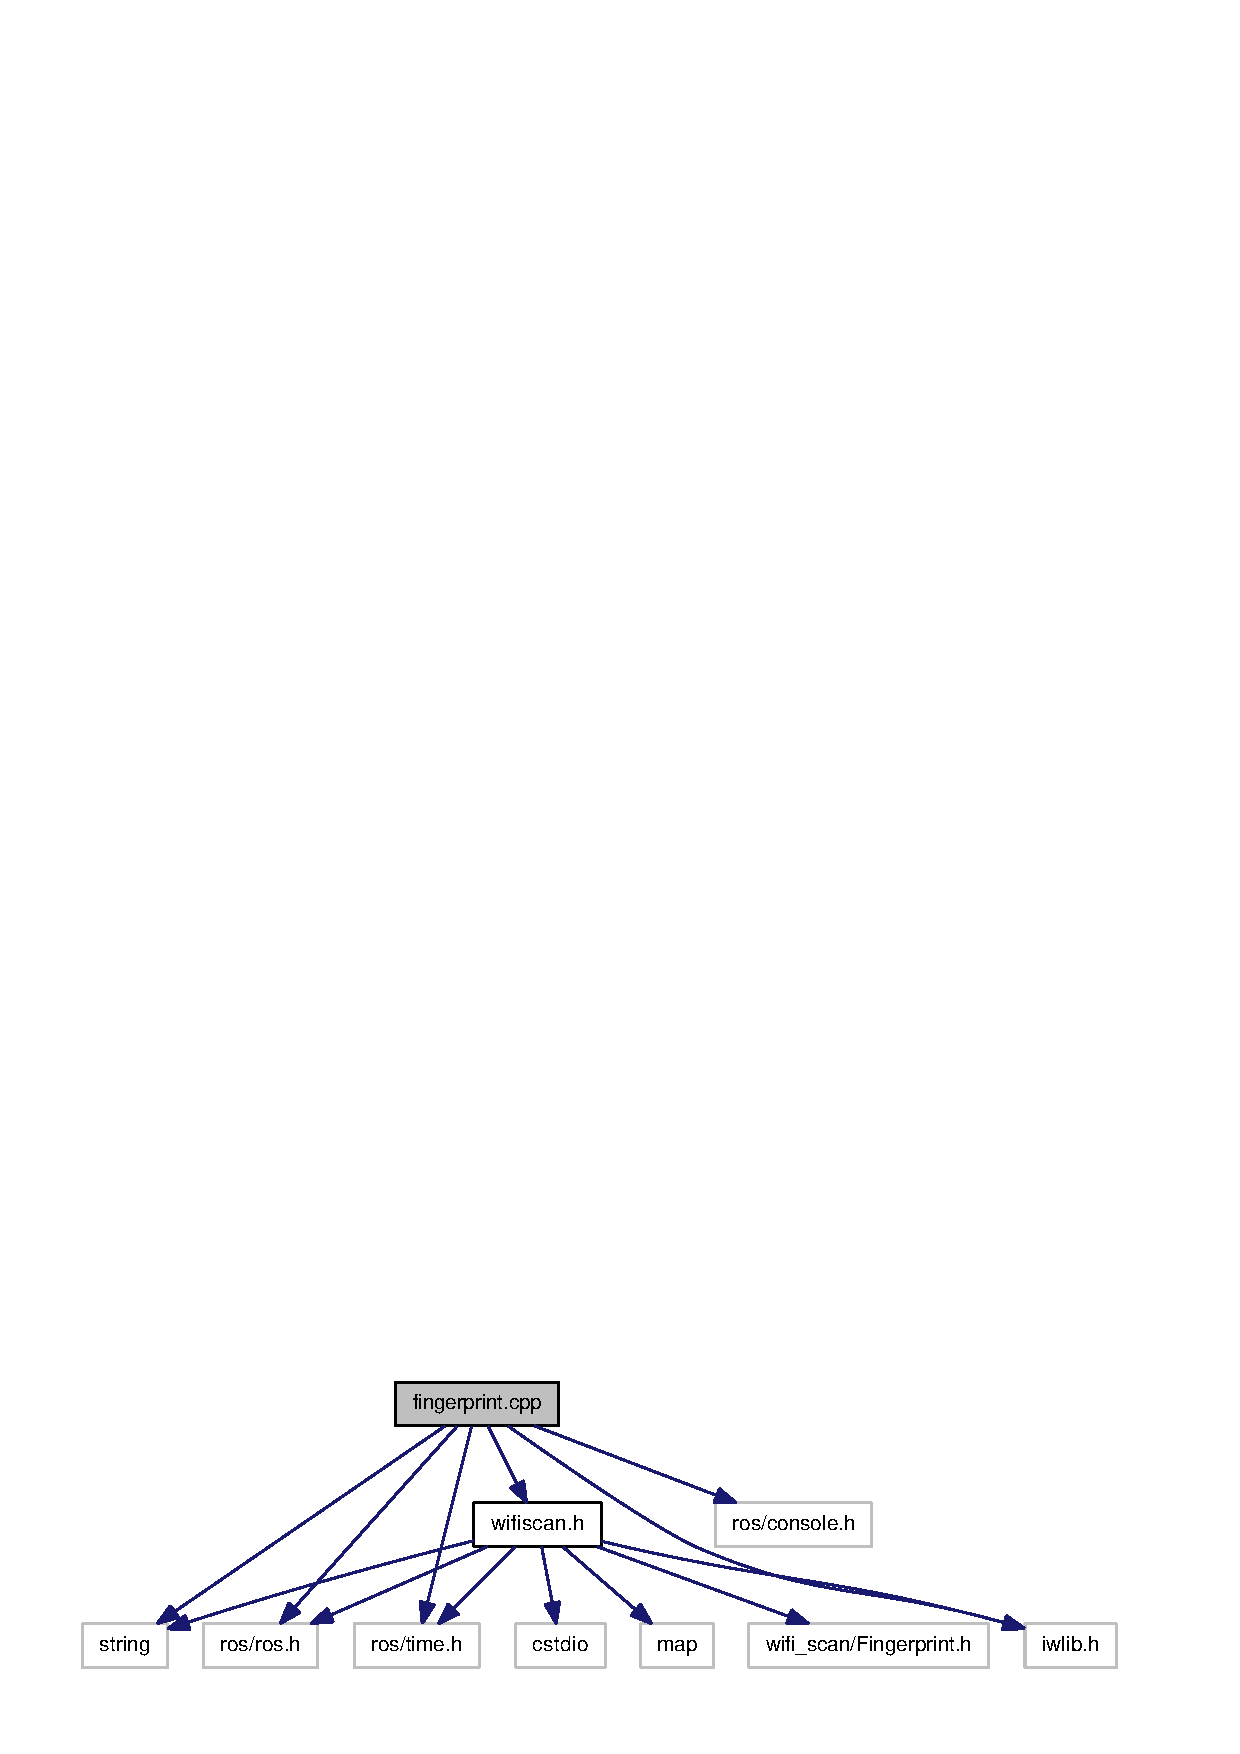
\includegraphics[width=350pt]{fingerprint_8cpp__incl}
\end{center}
\end{figure}
\subsection*{\-Functions}
\begin{DoxyCompactItemize}
\item 
int {\bf main} (int argc, char $\ast$$\ast$argv)
\begin{DoxyCompactList}\small\item\em \-Create a \-R\-O\-S node that publishes fingerprints. \end{DoxyCompactList}\end{DoxyCompactItemize}


\subsection{\-Function \-Documentation}
\index{fingerprint.\-cpp@{fingerprint.\-cpp}!main@{main}}
\index{main@{main}!fingerprint.cpp@{fingerprint.\-cpp}}
\subsubsection[{main}]{\setlength{\rightskip}{0pt plus 5cm}int {\bf main} (
\begin{DoxyParamCaption}
\item[{int}]{argc, }
\item[{char $\ast$$\ast$}]{argv}
\end{DoxyParamCaption}
)}\label{fingerprint_8cpp_a3c04138a5bfe5d72780bb7e82a18e627}


\-Create a \-R\-O\-S node that publishes fingerprints. 

\-This is the main function to set up the \-R\-O\-S node. 

\-Definition at line 34 of file fingerprint.\-cpp.


\section{mainpage.\-dox \-File \-Reference}
\label{mainpage_8dox}\index{mainpage.\-dox@{mainpage.\-dox}}

\section{wifiscan.\-cpp \-File \-Reference}
\label{wifiscan_8cpp}\index{wifiscan.\-cpp@{wifiscan.\-cpp}}
{\ttfamily \#include \char`\"{}wifiscan.\-h\char`\"{}}\*
\-Include dependency graph for wifiscan.\-cpp\-:\nopagebreak
\begin{figure}[H]
\begin{center}
\leavevmode
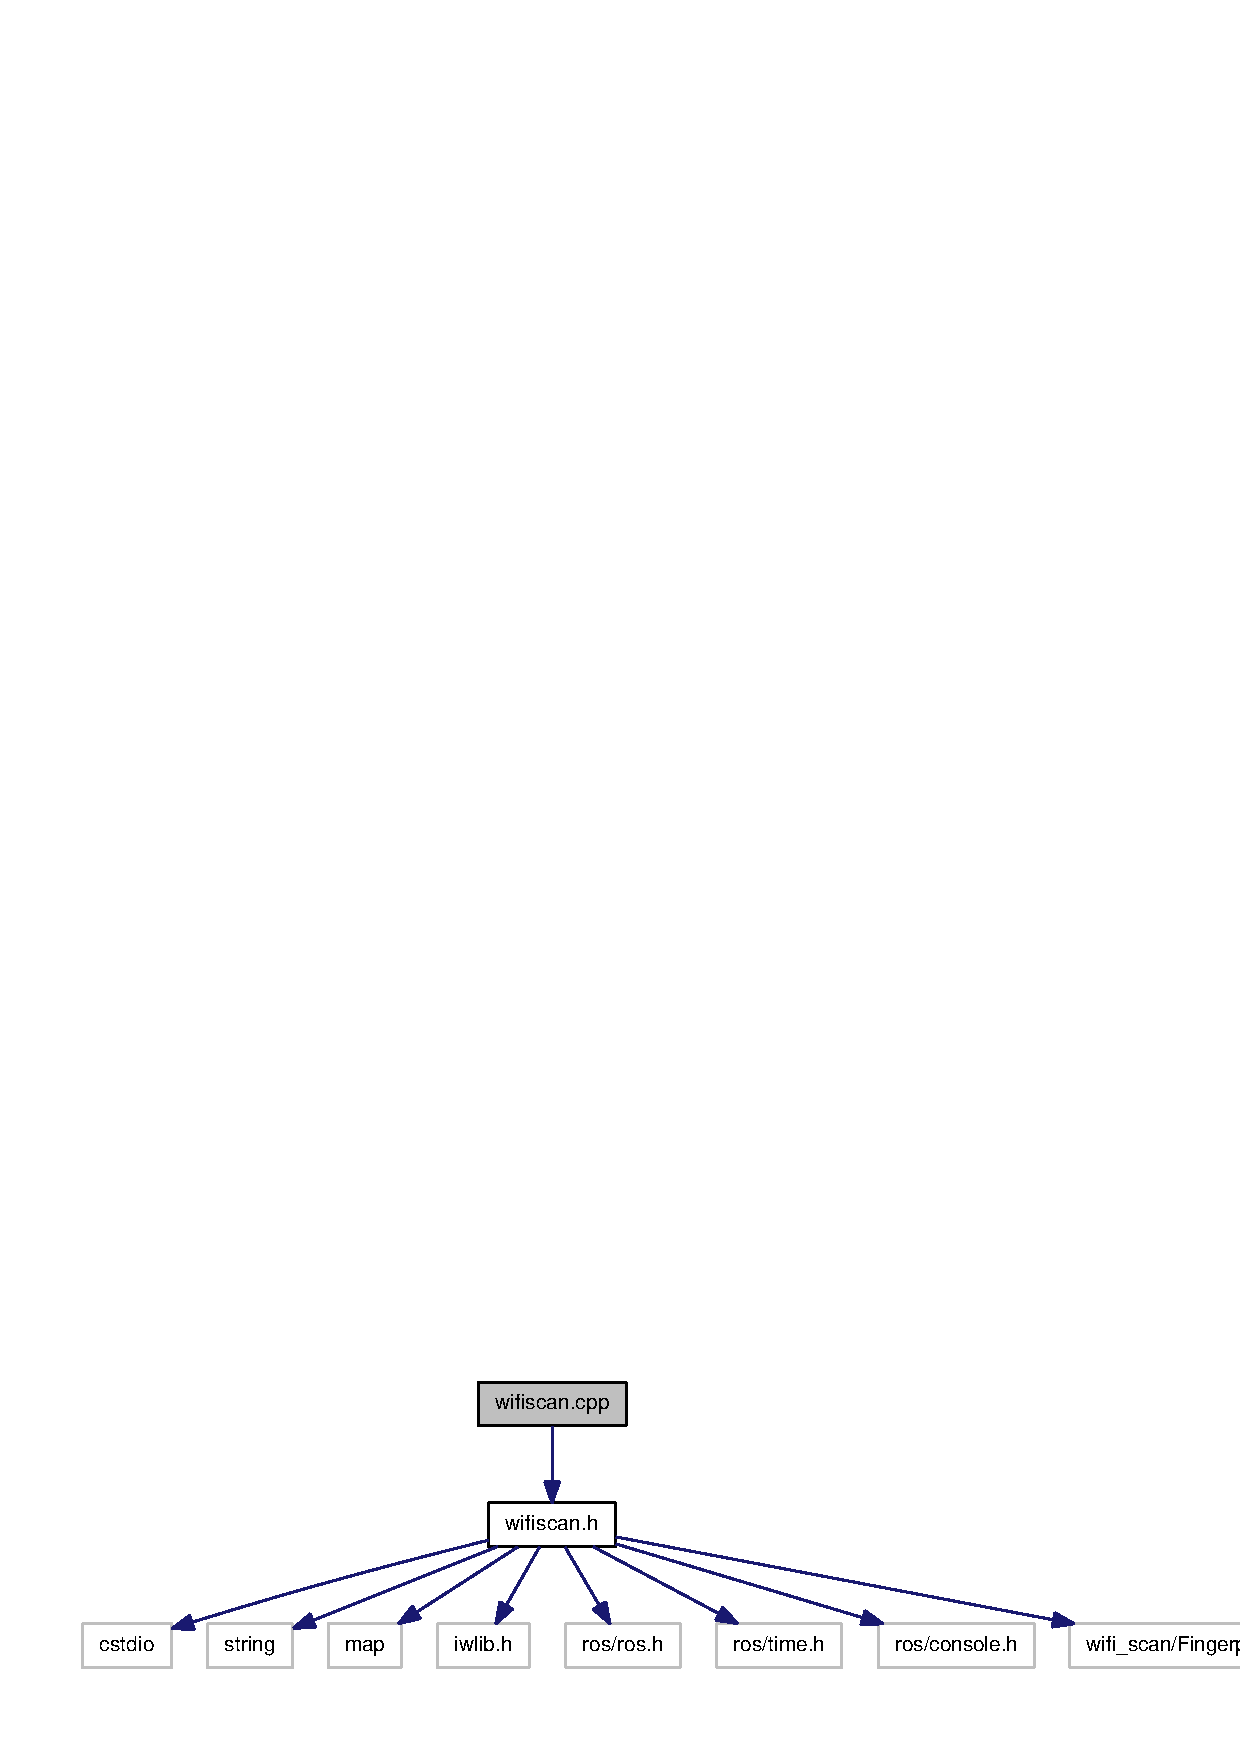
\includegraphics[width=350pt]{wifiscan_8cpp__incl}
\end{center}
\end{figure}

\section{wifiscan.\-h \-File \-Reference}
\label{wifiscan_8h}\index{wifiscan.\-h@{wifiscan.\-h}}
{\ttfamily \#include $<$cstdio$>$}\*
{\ttfamily \#include $<$string$>$}\*
{\ttfamily \#include $<$map$>$}\*
{\ttfamily \#include $<$iwlib.\-h$>$}\*
{\ttfamily \#include $<$ros/ros.\-h$>$}\*
{\ttfamily \#include $<$ros/time.\-h$>$}\*
{\ttfamily \#include $<$wifi\-\_\-scan/\-Fingerprint.\-h$>$}\*
\-Include dependency graph for wifiscan.\-h\-:\nopagebreak
\begin{figure}[H]
\begin{center}
\leavevmode
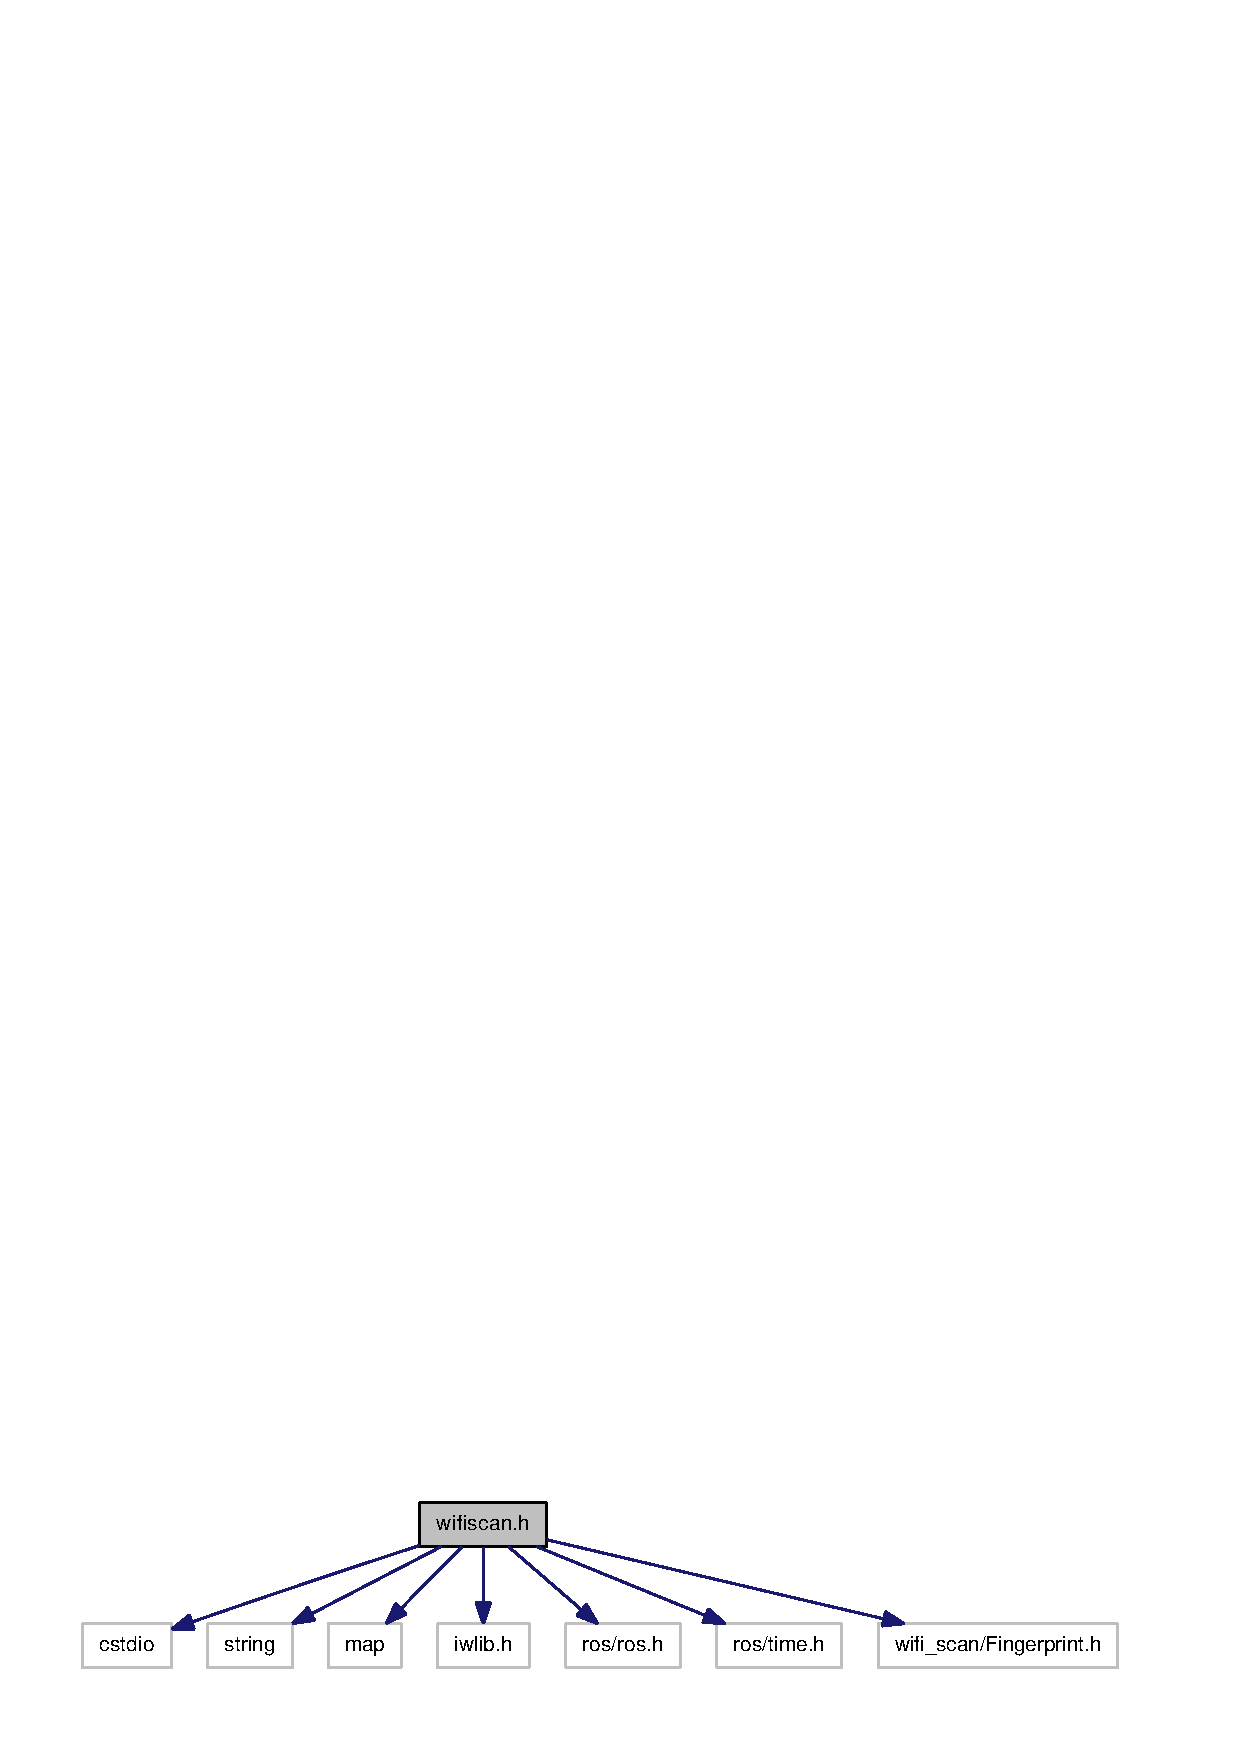
\includegraphics[width=350pt]{wifiscan_8h__incl}
\end{center}
\end{figure}
\-This graph shows which files directly or indirectly include this file\-:\nopagebreak
\begin{figure}[H]
\begin{center}
\leavevmode
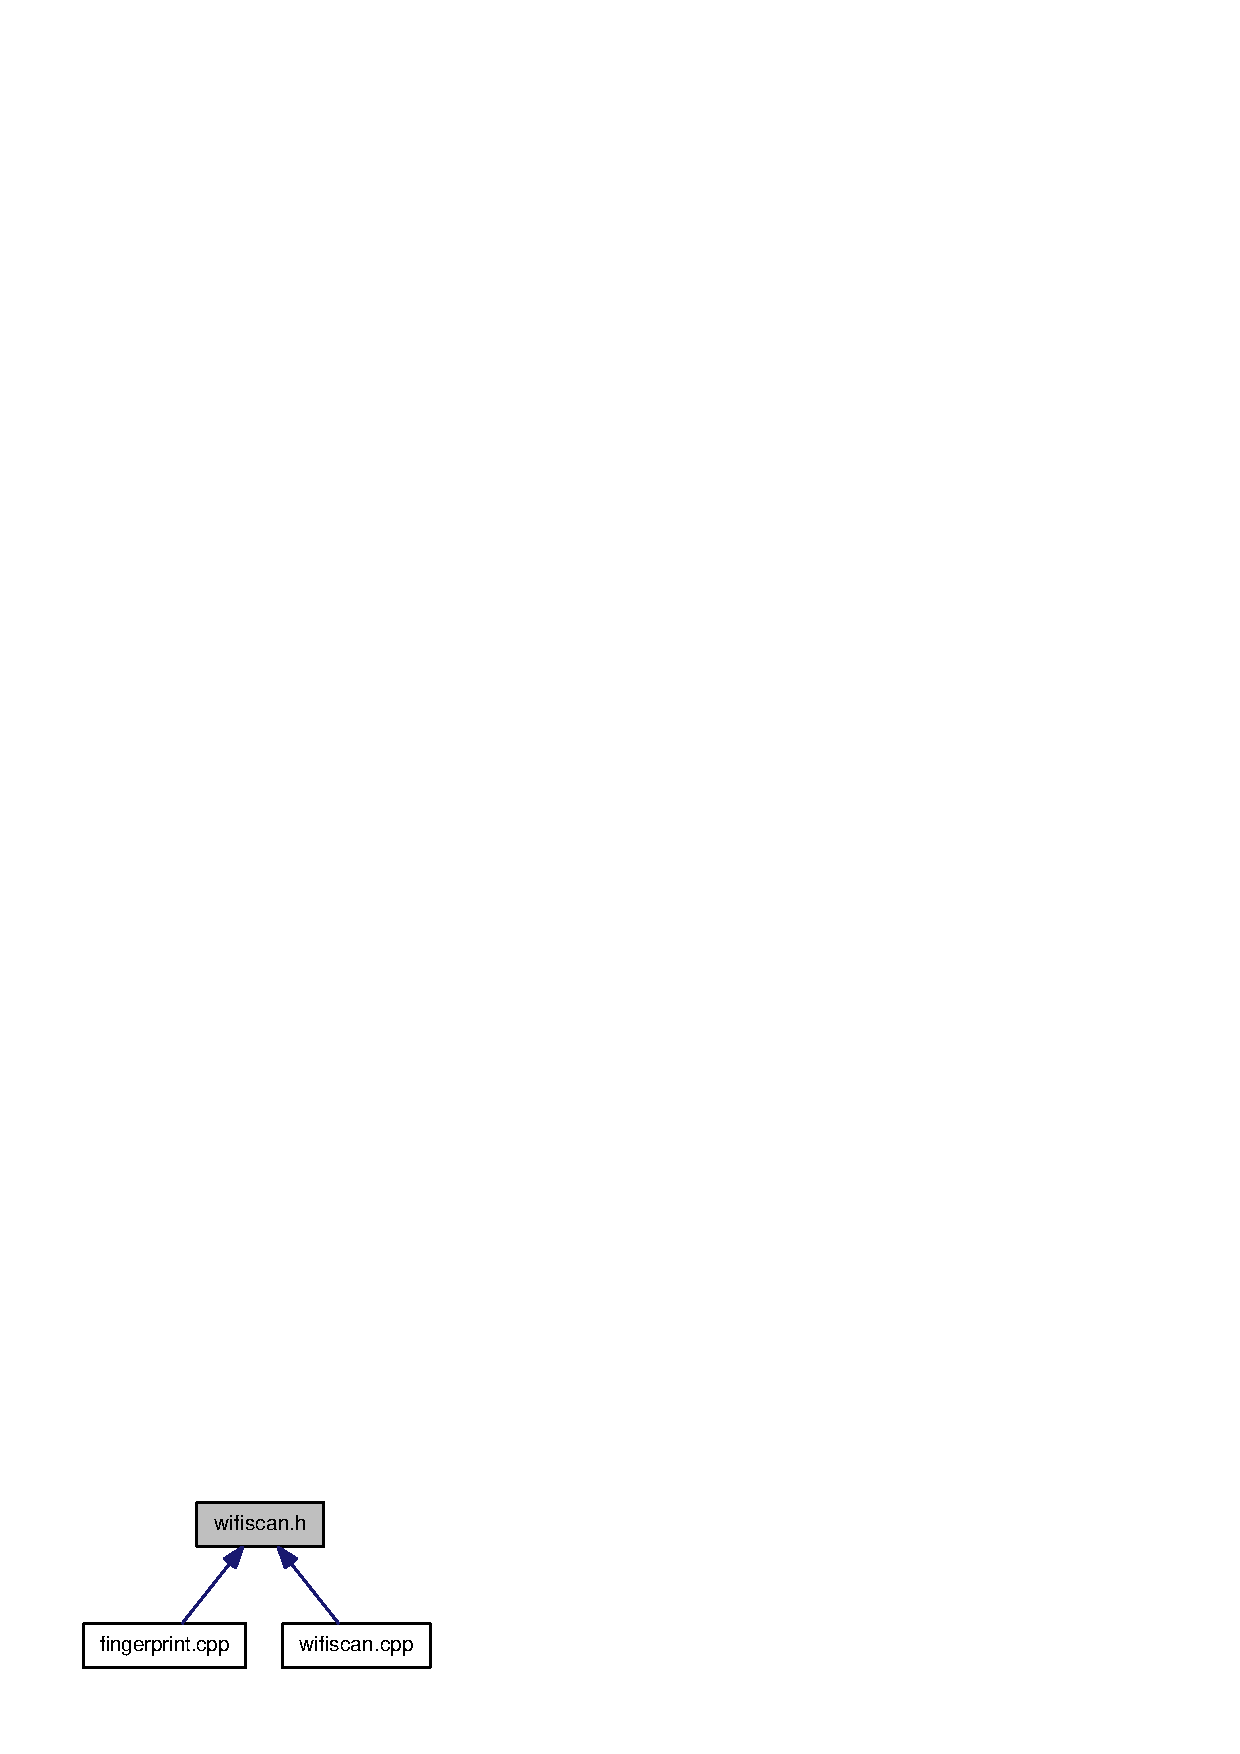
\includegraphics[width=210pt]{wifiscan_8h__dep__incl}
\end{center}
\end{figure}
\subsection*{\-Classes}
\begin{DoxyCompactItemize}
\item 
class {\bf \-Wifi\-Scan}
\begin{DoxyCompactList}\small\item\em \-The wifi\-\_\-scan main class. \end{DoxyCompactList}\end{DoxyCompactItemize}
\subsection*{\-Defines}
\begin{DoxyCompactItemize}
\item 
\#define {\bf \-W\-I\-F\-I\-S\-C\-A\-N\-\_\-\-E\-R\-R\-O\-R\-\_\-\-I\-N\-\_\-\-I\-W\-\_\-\-S\-C\-A\-N}~-\/2
\item 
\#define {\bf \-W\-I\-F\-I\-S\-C\-A\-N\-\_\-\-E\-R\-R\-O\-R\-\_\-\-O\-P\-E\-N\-I\-N\-G\-\_\-\-I\-O\-C\-T\-L\-\_\-\-S\-O\-C\-K\-E\-T}~-\/1
\end{DoxyCompactItemize}


\subsection{\-Define \-Documentation}
\index{wifiscan.\-h@{wifiscan.\-h}!\-W\-I\-F\-I\-S\-C\-A\-N\-\_\-\-E\-R\-R\-O\-R\-\_\-\-I\-N\-\_\-\-I\-W\-\_\-\-S\-C\-A\-N@{\-W\-I\-F\-I\-S\-C\-A\-N\-\_\-\-E\-R\-R\-O\-R\-\_\-\-I\-N\-\_\-\-I\-W\-\_\-\-S\-C\-A\-N}}
\index{\-W\-I\-F\-I\-S\-C\-A\-N\-\_\-\-E\-R\-R\-O\-R\-\_\-\-I\-N\-\_\-\-I\-W\-\_\-\-S\-C\-A\-N@{\-W\-I\-F\-I\-S\-C\-A\-N\-\_\-\-E\-R\-R\-O\-R\-\_\-\-I\-N\-\_\-\-I\-W\-\_\-\-S\-C\-A\-N}!wifiscan.h@{wifiscan.\-h}}
\subsubsection[{\-W\-I\-F\-I\-S\-C\-A\-N\-\_\-\-E\-R\-R\-O\-R\-\_\-\-I\-N\-\_\-\-I\-W\-\_\-\-S\-C\-A\-N}]{\setlength{\rightskip}{0pt plus 5cm}\#define {\bf \-W\-I\-F\-I\-S\-C\-A\-N\-\_\-\-E\-R\-R\-O\-R\-\_\-\-I\-N\-\_\-\-I\-W\-\_\-\-S\-C\-A\-N}~-\/2}\label{wifiscan_8h_a8ebfcf2ba8950fcab6d1e323f5017392}


\-Definition at line 35 of file wifiscan.\-h.

\index{wifiscan.\-h@{wifiscan.\-h}!\-W\-I\-F\-I\-S\-C\-A\-N\-\_\-\-E\-R\-R\-O\-R\-\_\-\-O\-P\-E\-N\-I\-N\-G\-\_\-\-I\-O\-C\-T\-L\-\_\-\-S\-O\-C\-K\-E\-T@{\-W\-I\-F\-I\-S\-C\-A\-N\-\_\-\-E\-R\-R\-O\-R\-\_\-\-O\-P\-E\-N\-I\-N\-G\-\_\-\-I\-O\-C\-T\-L\-\_\-\-S\-O\-C\-K\-E\-T}}
\index{\-W\-I\-F\-I\-S\-C\-A\-N\-\_\-\-E\-R\-R\-O\-R\-\_\-\-O\-P\-E\-N\-I\-N\-G\-\_\-\-I\-O\-C\-T\-L\-\_\-\-S\-O\-C\-K\-E\-T@{\-W\-I\-F\-I\-S\-C\-A\-N\-\_\-\-E\-R\-R\-O\-R\-\_\-\-O\-P\-E\-N\-I\-N\-G\-\_\-\-I\-O\-C\-T\-L\-\_\-\-S\-O\-C\-K\-E\-T}!wifiscan.h@{wifiscan.\-h}}
\subsubsection[{\-W\-I\-F\-I\-S\-C\-A\-N\-\_\-\-E\-R\-R\-O\-R\-\_\-\-O\-P\-E\-N\-I\-N\-G\-\_\-\-I\-O\-C\-T\-L\-\_\-\-S\-O\-C\-K\-E\-T}]{\setlength{\rightskip}{0pt plus 5cm}\#define {\bf \-W\-I\-F\-I\-S\-C\-A\-N\-\_\-\-E\-R\-R\-O\-R\-\_\-\-O\-P\-E\-N\-I\-N\-G\-\_\-\-I\-O\-C\-T\-L\-\_\-\-S\-O\-C\-K\-E\-T}~-\/1}\label{wifiscan_8h_ad1376d39aed25fbecc291d0d7dbad5f5}


\-Definition at line 34 of file wifiscan.\-h.


\printindex
\end{document}
